\chapter{De wereld waarnemen: de vijf zintuigen}\label{ch:g1:five-senses}

Ergens boven je zingt een vogel. Het brood ruikt warm. De stoeptegels
voelen koud door je sokken heen. Voordat de natuurkunde iets anders
doet, kijkt, luistert en voelt ze: dit hoofdstuk gaat over de wereld
\omterm{def:g1:five-senses:observation}{waarnemen} met de vijf \omterm{def:g1:five-senses:senses}{zintuigen} --- en over de streken die ze met ons
kunnen uithalen.

\section{De vijf zintuigen}

\begin{definition}[De vijf zintuigen]\label{def:g1:five-senses:senses}
Een \emph{zintuig}\index{zintuig} is een manier waarop je lichaam iets
over de wereld te weten komt. We hebben er vijf:
\begin{enumerate}
  \item \emph{zien}\index{zien} --- de ogen zien licht, kleuren en
        vormen;
  \item \emph{horen}\index{horen} --- de oren horen geluiden;
  \item \emph{voelen}\index{voelen} --- de huid voelt ruw of glad,
        warm of koud;
  \item \emph{ruiken}\index{ruiken} --- de neus ruikt het warme brood;
  \item \emph{proeven}\index{proeven} --- de tong proeft zoet, zout,
        zuur.
\end{enumerate}
\end{definition}

\begin{omfigure}
\begin{tikzpicture}[scale=0.8]
  \foreach \x/\name in {0/zien, 2.4/horen, 4.8/voelen, 7.2/ruiken,
      9.6/proeven} {
    \draw[thick, omDef] (\x,0) circle (0.9);
    \node[below, font=\small] at (\x,-1.1) {\name};
  }
  % eye
  \draw[thick] (0,0) ellipse (0.55 and 0.3);
  \fill[omDef] (0,0) circle (0.18);
  \fill (0,0) circle (0.09);
  \fill[white] (0.06,0.07) circle (0.03);
  % ear: outer contour over the top, down to the lobe, plus inner ridge
  \draw[thick] (2.12,0.3)
    .. controls (2.1,0.62) and (2.42,0.72) .. (2.66,0.52)
    .. controls (2.88,0.32) and (2.86,-0.08) .. (2.68,-0.32)
    .. controls (2.55,-0.5) and (2.4,-0.62) .. (2.26,-0.6)
    .. controls (2.1,-0.58) and (2.06,-0.42) .. (2.14,-0.32);
  \draw[thick] (2.24,0.28)
    .. controls (2.26,0.46) and (2.5,0.5) .. (2.6,0.32)
    .. controls (2.7,0.12) and (2.64,-0.08) .. (2.5,-0.16);
  % hand print: palm and five fingers
  \fill[omDef!30] (4.72,-0.22) ellipse (0.34 and 0.28);
  \draw[thick] (4.72,-0.22) ellipse (0.34 and 0.28);
  \foreach \a/\r in {135/0.5, 108/0.56, 84/0.58, 60/0.54} {
    \fill[omDef!30] (4.72,-0.22) ++(\a:\r)
      ellipse [x radius=0.085, y radius=0.17, rotate=\a-90];
    \draw[thick] (4.72,-0.22) ++(\a:\r)
      ellipse [x radius=0.085, y radius=0.17, rotate=\a-90];
  }
  \fill[omDef!30] (4.72,-0.22) ++(170:0.46)
    ellipse [x radius=0.08, y radius=0.14, rotate=60];
  \draw[thick] (4.72,-0.22) ++(170:0.46)
    ellipse [x radius=0.08, y radius=0.14, rotate=60];
  % nose in profile: brow, bridge sloping down-left, rounded tip,
  % nostril wing curling back
  \draw[thick] (7.5,0.62)
    .. controls (7.32,0.4) and (7.16,0.14) .. (7.1,-0.08)
    .. controls (7.05,-0.26) and (7.14,-0.4) .. (7.3,-0.4)
    .. controls (7.4,-0.4) and (7.46,-0.34) .. (7.46,-0.26);
  \draw[thick] (7.46,-0.26)
    .. controls (7.56,-0.3) and (7.6,-0.42) .. (7.5,-0.48)
    .. controls (7.42,-0.53) and (7.3,-0.49) .. (7.28,-0.42);
  \fill (7.38,-0.44) ellipse (0.05 and 0.033);
  % lips
  \draw[thick] (9.2,0.06) .. controls (9.4,0.24) and (9.52,0.12) ..
    (9.6,0.16) .. controls (9.68,0.12) and (9.8,0.24) .. (10.0,0.06);
  \draw[thick] (9.2,0.06) .. controls (9.45,-0.28) and (9.75,-0.28)
    .. (10.0,0.06);
  \draw[thick] (9.34,0.02) .. controls (9.6,-0.08) .. (9.86,0.02);
\end{tikzpicture}

{\small De vijf \omterm{def:g1:five-senses:senses}{zintuigen}: oog, oor, hand, neus, tong --- vijf deuren
tussen de wereld en jou.}
\end{omfigure}

\begin{example}[Eén appel, vijf zintuigen]\label{ex:g1:five-senses:apple}
Bij het eten van een appel doen alle \omterm{def:g1:five-senses:senses}{zintuigen} mee: je \emph{ziet}
zijn rode schil, je \emph{voelt} hem glad en rond in je hand, je
\emph{hoort} het kraken, je \emph{ruikt} zijn geur, je \emph{proeft}
zijn zoete sap. Vijf \omterm{def:g1:five-senses:senses}{zintuigen}, één appel.
\end{example}

\begin{omfigure}
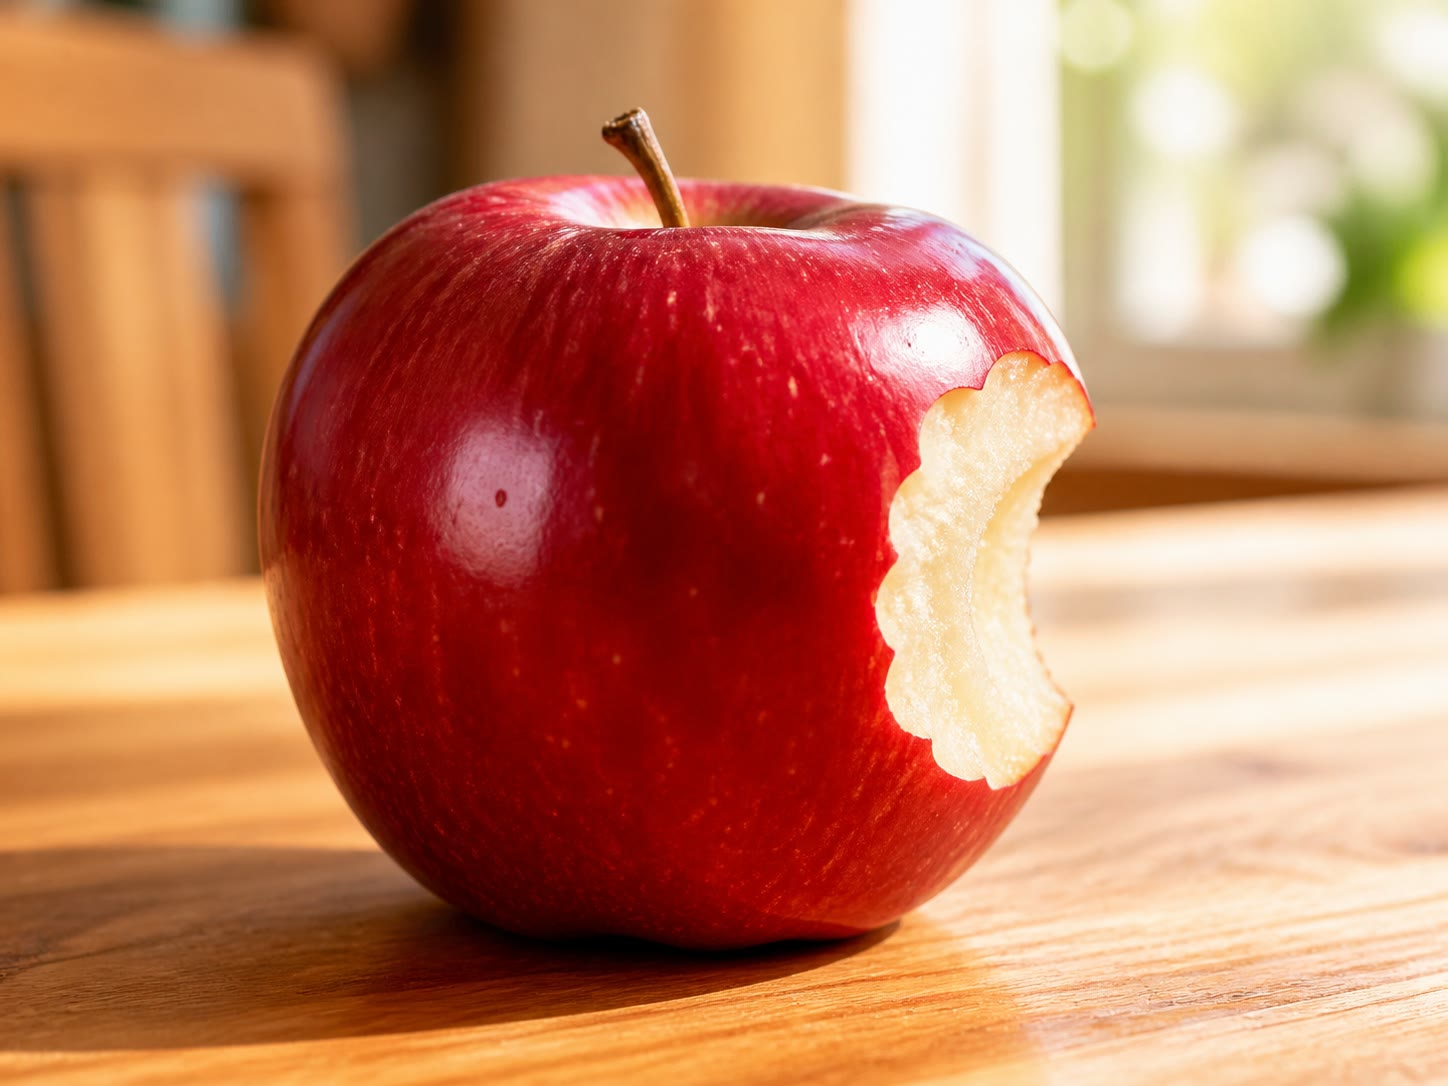
\includegraphics[width=0.52\linewidth]{images/book1/ai/g1-five-senses-apple.jpg}

{\small Eén appel voor alle vijf de \omterm{def:g1:five-senses:senses}{zintuigen}: de ogen zien zijn rood, de hand voelt zijn gladde schil, de oren hoorden het kraken van de ontbrekende hap, de neus ruikt zijn geur, de tong houdt de smaak vast.}
\end{omfigure}

\begin{example}[Probeer het: de geluidenwandeling]\label{ex:g1:five-senses:sounds}
Ga stil zitten, doe je ogen dicht en tel een tijdje de geluiden om je
heen: een auto, een stem, de wind, je eigen ademhaling. Met je ogen
dicht merken je oren geluiden op die je door je drukke ogen miste. De
meeste mensen vinden $4$ of $5$ geluiden die ze eerder niet hadden
gehoord.
\end{example}

\begin{remark}[Zintuigen die ons beschermen]\label{rem:g1:five-senses:danger}
De \omterm{def:g1:five-senses:senses}{zintuigen} zijn ook wachters. De neus ruikt rook voordat de ogen
vuur zien; de huid trekt de hand terug van een hete pan; een bittere
smaak waarschuwt: ``dit niet doorslikken''. Ruik of proef nooit
expres aan iets onbekends: vraag het eerst aan een volwassene. De
wachters werken het best als we voorzichtig met ze omgaan.
\end{remark}

\section{Zorgvuldig waarnemen}

Kijken is nog geen \omterm{def:g1:five-senses:observation}{waarnemen}. Iedereen heeft weleens een
lieveheersbeestje \emph{gezien}; wie kan zeggen hoeveel pootjes het
heeft?

\begin{definition}[Waarneming]\label{def:g1:five-senses:observation}
\emph{Waarnemen}\index{waarnemen} is je \omterm{def:g1:five-senses:senses}{zintuigen} zorgvuldig en met
opzet gebruiken om een vraag te beantwoorden --- en daarna precies
vertellen of tekenen wat je hebt gemerkt, niet wat je verwachtte. Een
\emph{waarneming}\index{waarneming} is wat zorgvuldig kijken heeft
gevonden.
\end{definition}

\begin{method}[Zo neem je waar]\label{met:g1:five-senses:how}
\begin{enumerate}
  \item Kies een vraag: \emph{hoeveel pootjes heeft het
        lieveheersbeestje?}
  \item kijk (of luister, of voel) rustig, zonder haast;
  \item zeg met precieze woorden wat je merkt: niet ``het is klein'',
        maar ``het is kleiner dan mijn nagel'';
  \item teken of vertel het, zodat iemand anders het kan nakijken.
\end{enumerate}
Een goede \omterm{def:g1:five-senses:observation}{waarneming} kan een vriend nakijken: als jullie allebei
kijken, moeten jullie allebei $6$ pootjes vinden.
\end{method}

\begin{example}[Precieze woorden]\label{ex:g1:five-senses:words}
Vergelijk ``de steen is leuk'' met ``de steen is grijs, glad, rond en
kouder dan mijn hand''. De tweede zin is een
\omterm{def:g1:five-senses:observation}{waarneming}: een ander kind kan die steen uit een hele mand
halen.
\end{example}

\begin{omfigure}
\begin{tikzpicture}[scale=0.8]
  % six legs, three per side
  \draw[thick] (1.32,-0.45) -- ++(-30:0.45);
  \draw[thick] (0.9,-0.76) -- ++(-55:0.45);
  \draw[thick] (0.38,-0.92) -- ++(-75:0.45);
  \draw[thick] (-1.32,-0.45) -- ++(210:0.45);
  \draw[thick] (-0.9,-0.76) -- ++(235:0.45);
  \draw[thick] (-0.38,-0.92) -- ++(255:0.45);
  % body, wing split, spots
  \draw[thick, fill=omDef!12] (0,0) ellipse (1.5 and 0.95);
  \draw[thick, omDef] (0,0.95) -- (0,-0.95);
  \fill[omThm] (-0.55,0.3) circle (0.13);
  \fill[omThm] (-0.85,-0.25) circle (0.13);
  \fill[omThm] (0.5,0.4) circle (0.13);
  \fill[omThm] (0.75,-0.25) circle (0.13);
  % head and antennae
  \fill[omDef] (1.55,0) circle (0.3);
  \draw[thick] (1.75,0.18) .. controls (2.0,0.35) .. (2.1,0.55);
  \draw[thick] (1.78,-0.14) .. controls (2.05,-0.28) .. (2.18,-0.42);
  \node[right, font=\small] at (2.8,0.5)
    {Hoeveel stippen? Hoeveel pootjes?};
  \node[right, font=\small] at (2.8,-0.5)
    {Kijk rustig, en tel dan.};
\end{tikzpicture}

{\small Een lieveheersbeestje \omterm{def:g1:five-senses:observation}{waarnemen}: zorgvuldige ogen tellen bij
dit exemplaar $4$ stippen --- en altijd $6$ pootjes.}
\end{omfigure}

\section{Als de zintuigen bedrogen worden}

De \omterm{def:g1:five-senses:senses}{zintuigen} zijn prachtig, maar je kunt ze voor de gek houden. Juist
daarom leren we in de volgende hoofdstukken \emph{meten}.

\begin{example}[Twee lijnen]\label{ex:g1:five-senses:lines}
Welke lijn is op de tekening hieronder langer? Bijna iedereen zegt
``de bovenste''. Kijk nu na met een touwtje: de twee lijnen zijn
precies even lang. De ogen lieten zich bedriegen door de pijlpunten.
\end{example}

\begin{omfigure}
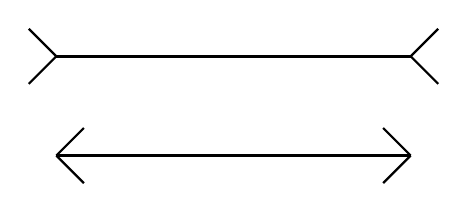
\begin{tikzpicture}[scale=0.9]
  \draw[very thick] (0,1.4) -- (5,1.4);
  \draw[thick] (0,1.4) -- ++(135:0.55) (0,1.4) -- ++(-135:0.55);
  \draw[thick] (5,1.4) -- ++(45:0.55) (5,1.4) -- ++(-45:0.55);
  \draw[very thick] (0,0) -- (5,0);
  \draw[thick] (0,0) -- ++(45:0.55) (0,0) -- ++(-45:0.55);
  \draw[thick] (5,0) -- ++(135:0.55) (5,0) -- ++(-135:0.55);
\end{tikzpicture}

{\small De beroemde truc met de pijlpunten: beide lijnen zijn even
lang. Kijk het na met een touwtje!}
\end{omfigure}

\begin{example}[Probeer het: drie kommen]\label{ex:g1:five-senses:bowls}
Vraag een volwassene om drie kommen water klaar te zetten: één koele,
één lauwe en één aangenaam warme. Houd je ene hand in de koele kom en
je andere in de warme kom terwijl je rustig tot $20$ telt. Steek dan
allebei je handen in de kom in het midden: hetzelfde water voelt warm
voor de ene hand en koel voor de andere! Op je gevoel alleen kun je
niet vertrouwen als het om warm en koud gaat --- het volgende
hoofdstuk pakt precies dat probleem op.
\end{example}

\begin{remark}[Hulpjes voor de zintuigen]\label{rem:g1:five-senses:tools}
Mensen maken gereedschap dat de \omterm{def:g1:five-senses:senses}{zintuigen} helpt: een bril en een
vergrootglas helpen de ogen, de stethoscoop van de dokter helpt de
oren. Verderop in dit boek doet gereedschap dat \emph{instrumenten}
heet het nog beter: dat maakt van kijken en voelen een kwestie van
tellen en meten, en tellen is veel moeilijker voor de gek te houden.
\end{remark}

\section{Oefeningen}

\begin{exercise}[$\star$]\label{exo:g1:five-senses:1}
Noem de vijf \omterm{def:g1:five-senses:senses}{zintuigen}, en bij elk het lichaamsdeel dat het werk
doet.
\end{exercise}

\begin{exercise}[$\star$]\label{exo:g1:five-senses:2}
Welk \omterm{def:g1:five-senses:senses}{zintuig} vertelt je: (a) dat de radio aanstaat? (b) dat de soep
te zout is? (c) dat je trui kriebelt? (d) dat het licht uitging?
\end{exercise}

\begin{exercise}[$\star$]\label{exo:g1:five-senses:3}
In een andere kamer bakt een cake in de oven, met de deur dicht.
Welk \omterm{def:g1:five-senses:senses}{zintuig} vindt hem het eerst? Welke \omterm{def:g1:five-senses:senses}{zintuigen} gebruik je als je
eindelijk een stuk krijgt?
\end{exercise}

\begin{exercise}[$\star$]\label{exo:g1:five-senses:4}
Doe de geluidenwandeling van \cref{ex:g1:five-senses:sounds}: ogen
dicht, tel de geluiden om je heen. Hoeveel hoorde je er? Welk geluid
verraste je?
\end{exercise}

\begin{exercise}[$\star$]\label{exo:g1:five-senses:5}
Geef een \omterm{def:g1:five-senses:observation}{waarneming} van je schoen met drie precieze woorden, zoals in
\cref{ex:g1:five-senses:words}. ``Leuk'' en ``mooi'' mogen niet!
\end{exercise}

\begin{exercise}[$\star$]\label{exo:g1:five-senses:6}
Ana zegt: ``De kat is zacht.'' Bob zegt: ``De kat is de beste kat.''
Welke zin is een \omterm{def:g1:five-senses:observation}{waarneming}, en welk \omterm{def:g1:five-senses:senses}{zintuig} heeft hem gemaakt? Wat is
de andere zin?
\end{exercise}

\begin{exercise}[$\star$]\label{exo:g1:five-senses:7}
Welk \omterm{def:g1:five-senses:senses}{zintuig} waarschuwt je voor elk gevaar: (a) rook ergens in het
huis; (b) een pan die te heet is om vast te pakken; (c) een auto die
van achteren aankomt?
\end{exercise}

\begin{exercise}[$\star$]\label{exo:g1:five-senses:8}
Een vriend doet zijn ogen dicht. Jij legt één voor één een lepel, een
spons en een kiezelsteen voor hem neer. Kan hij ze alle drie alleen
op de tast benoemen? Welke was het makkelijkst te herkennen?
\end{exercise}

\begin{exercise}[$\star\star$]\label{exo:g1:five-senses:9}
Kijk naar de twee lijnen van \cref{ex:g1:five-senses:lines}. Leg een
vriend uit hoe je zeker weet welke lijn langer is, zonder op je ogen
te vertrouwen. Kan je manier ook een lijn met een kronkelig touwtje
vergelijken?
\end{exercise}
